%\documentclass[a4paper,10pt,english]{amsart}
\documentclass[a4paper,10pt,english]{article}
%\documentclass[12pt,preprint]{aastex}
\usepackage[utf8]{inputenc}
\usepackage[margin=0.3in]{geometry} % narrow margins
\usepackage{graphicx}
\usepackage{float}
\usepackage{amsmath}
\usepackage{epsfig,floatflt}
\usepackage{hyperref}
\usepackage{listings}
\usepackage[table,xcdraw]{xcolor}
\usepackage{booktabs}
\usepackage{amsmath,graphicx,varioref,verbatim,amsfonts,geometry,amssymb,dsfont,blindtext}
\hypersetup{colorlinks=true}
\usepackage{xcolor}
\usepackage{hhline}
\definecolor{LightGray}{gray}{0.95}
\definecolor{dkgreen}{rgb}{0,0.6,0}
\definecolor{gray}{rgb}{0.5,0.5,0.5}
\definecolor{mauve}{rgb}{0.58,0,0.82}
\definecolor{mygray}{rgb}{0.9,0.9,0.9}
\definecolor{LightGray}{gray}{0.95}
\lstset{frame=tb,
	language=Python,
	aboveskip=3mm,
	belowskip=3mm,
	showstringspaces=false,
	columns=flexible,
	basicstyle={\small\ttfamily},
	numbers=none,
	numberstyle=\tiny\color{gray},
	keywordstyle=\color{blue},
	commentstyle=\color{dkgreen},
	stringstyle=\color{mauve},
	backgroundcolor=\color{mygray},
	breaklines=true,
	postbreak=\mbox{\textcolor{red}{$\hookrightarrow$}\space}
	%breakatwhitespace=true,
	%tabsize=3
}



\begin{document}
%\twocolumn

\title{FYS-STK4155 Project 1}
\author{Bendik Steinsvåg Dalen \& Gabriel Sigurd Cabrera}
\maketitle

\begin{abstract}

\end{abstract}

\section{Introduction}
\label{sec:introduction}

yvycjyukioyjfchdxcgfjhbk
\section{Data}
\label{sec:data}

\section{Method}
\label{sec:method}

\section{Results}
\label{sec:results}

%Part a and b:

\begin{figure}[h!]
	\centering 
	%Scale angir størrelsen på bildet. Bildefilen må ligge i %samme mappe som tex-filen. 
	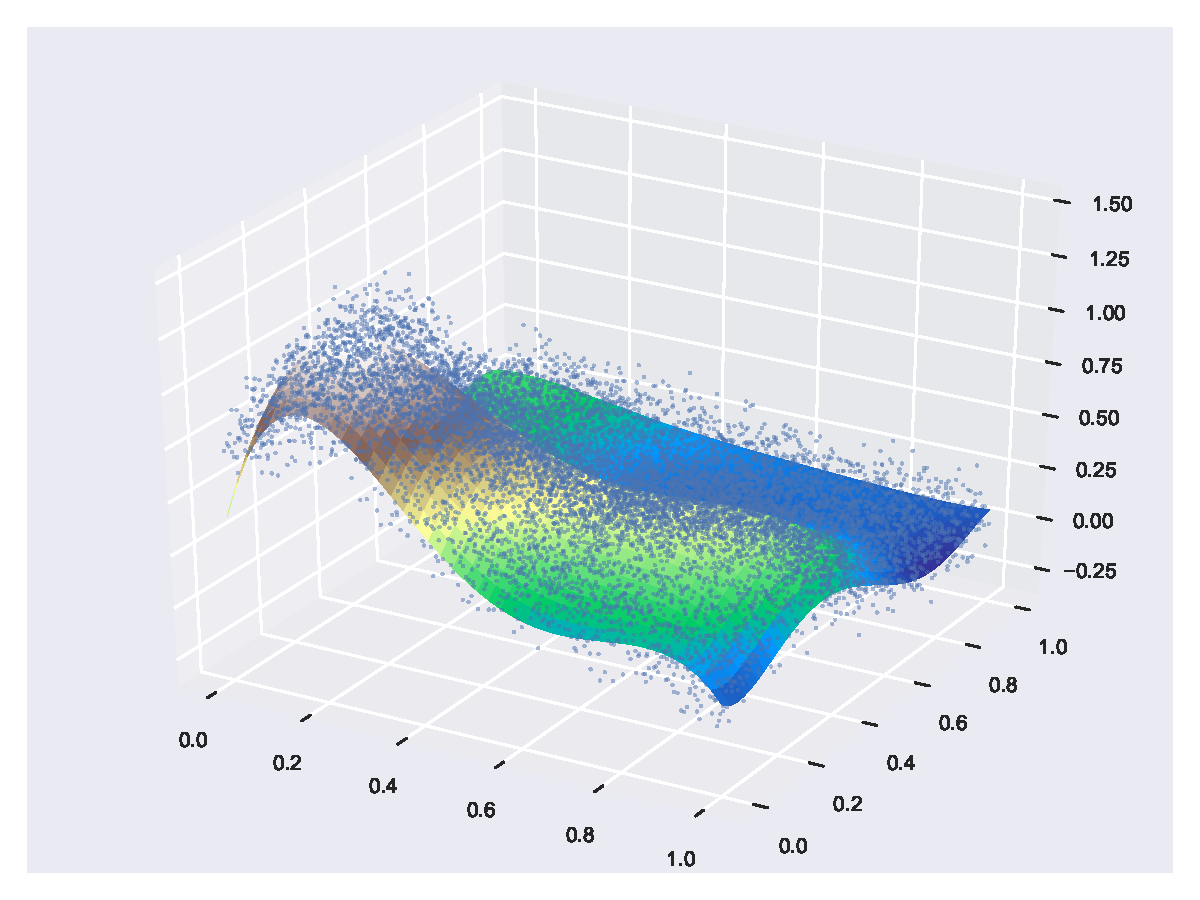
\includegraphics[scale=0.6]{../results/part_a_reg.pdf}
	\caption{The resulting function after performing a standard least square regression analysis using polynomials in x and y up to fifth order on the Franke function}
	%Label gjør det enkelt å referere til ulike bilder.
	\label{part_a}
\end{figure}

\begin{table}[htbp]
%	\centering
	\begin{tabular}{|>{\columncolor[HTML]{EFEFEF}}c|c|c|c|c|c|c|c|c|c|c|c|c|c|c|c|c|c|}
		\hline
		\cellcolor[HTML]{9B9B9B} & \cellcolor[HTML]{EFEFEF}$\beta_0$ & \cellcolor[HTML]{EFEFEF}$\beta_1$ & \cellcolor[HTML]{EFEFEF}$\beta_2$ & \cellcolor[HTML]{EFEFEF}$\beta_3$ & \cellcolor[HTML]{EFEFEF}$\beta_4$ & \cellcolor[HTML]{EFEFEF}$\beta_5$ & \cellcolor[HTML]{EFEFEF}$\beta_6$ & \cellcolor[HTML]{EFEFEF}$\beta_7$ & \cellcolor[HTML]{EFEFEF}$\beta_8$ & \cellcolor[HTML]{EFEFEF}$\beta_9$ & \cellcolor[HTML]{EFEFEF}$\beta_{10}$ & \cellcolor[HTML]{EFEFEF}$\beta_{11}$ & \cellcolor[HTML]{EFEFEF}$\beta_{12}$ & \cellcolor[HTML]{EFEFEF}$\beta_{13}$ & \cellcolor[HTML]{EFEFEF}$\beta_{14}$ & \cellcolor[HTML]{EFEFEF}$\beta_{15}$ & \cellcolor[HTML]{EFEFEF}$\beta_{16}$  \\ \hline
		SLS & 0.00789 & 0.322 & 2.46 & 4.81 & 5.61 & 1.76 & 0.322 & 1.85 & 4.3 & 5.97 & 2.83 & 2.46 & 4.3 & 5.97 & 4.23 & 4.81 & 5.97  \\ \hline
		$k$-fold & 0.0321 & 4.03 & 94 & 474 & 517 & 79.5 & 4.03 & 57.3 & 260 & 301 & 60.1 & 93.9 & 260 & 261 & 57.1 & 474 & 301 \\ \hline
	\end{tabular}

	\begin{tabular}{|>{\columncolor[HTML]{EFEFEF}}c|c|c|c|c|}
		\hline
		\cellcolor[HTML]{9B9B9B} & \cellcolor[HTML]{EFEFEF}$\beta_{17}$ & \cellcolor[HTML]{EFEFEF}$\beta_{18}$ & \cellcolor[HTML]{EFEFEF}$\beta_{19}$ & \cellcolor[HTML]{EFEFEF}$\beta_{20}$ \\ \hline
		SLS & 4.23 & 5.61 & 2.83 & 1.76  \\ \hline
		$k$-fold &  57.1 & 517 & 60.1 & 79.5  \\ \hline
	\end{tabular}
	\caption{The variance of $\beta$ for the standard least square regression and for $k$-fold validation}
\end{table}

\begin{table}[htbp]
	\centering
	\begin{tabular}{|
			>{\columncolor[HTML]{EFEFEF}}c |c|c|}
		\hline
		\cellcolor[HTML]{9B9B9B} & \cellcolor[HTML]{EFEFEF}MSE & \cellcolor[HTML]{EFEFEF}$R^2$ \\ \hline
		SLS                      & 0.015                       & 0.84                          \\ \hline
		$k$-fold                 & 0.012                       & 0.87                          \\ \hline
	\end{tabular}
	\caption{MSE and R2 for a and b}
\end{table}
%\begin{table}[htbp]
%	\centering
%	\begin{tabular}{|c|c|c|}
%		\hline
%		& MSE & \\ \hline
%		SLS                      & 0.015                       & 0.84                          \\ \hline
%		$k$-fold                 & 0.012                       & 0.87                          \\ \hline
%	\end{tabular}
%	\caption{MSE and R2 for a and b}
%\end{table}


%Part d:


\begin{figure}[h!]
	\centering 
	%Scale angir størrelsen på bildet. Bildefilen må ligge i %samme mappe som tex-filen. 
	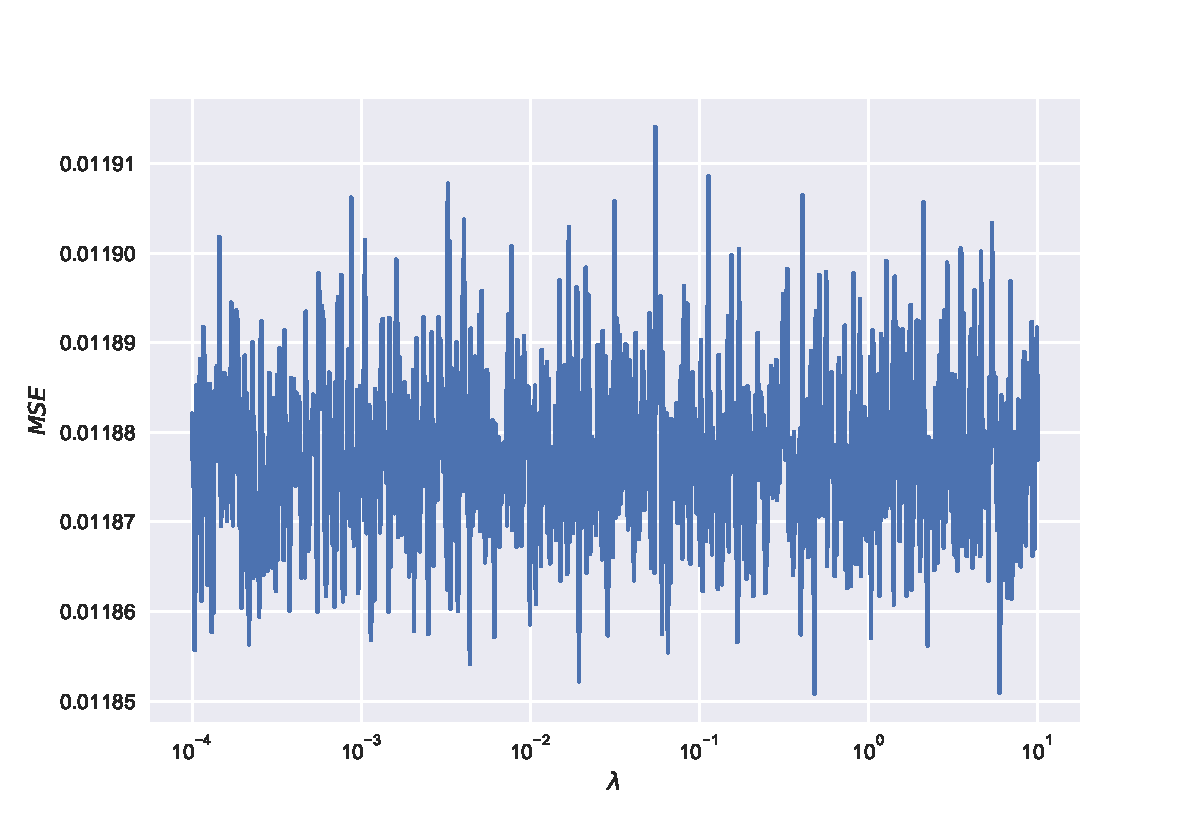
\includegraphics[scale=0.6]{../results/part_d_reg_MSE.pdf}
	\caption{The Mean Squared Error for the Ridge method for different values of $\lambda$}
	%Label gjør det enkelt å referere til ulike bilder.
	\label{part_d_MSE}
\end{figure}

\begin{figure}[h!]
	\centering 
	%Scale angir størrelsen på bildet. Bildefilen må ligge i %samme mappe som tex-filen. 
	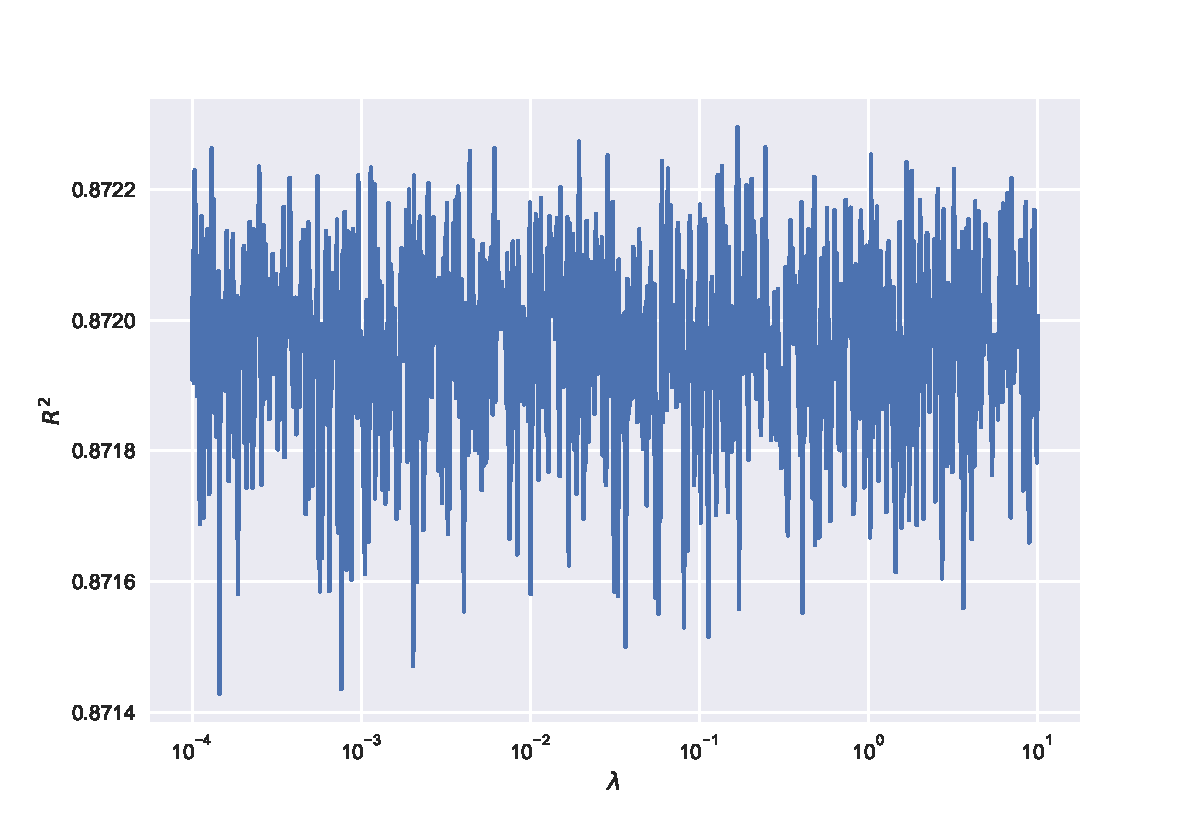
\includegraphics[scale=0.6]{../results/part_d_reg_R2.pdf}
	\caption{$R^2$-score for the Ridge method for different values of $\lambda$}
	%Label gjør det enkelt å referere til ulike bilder.
	\label{part_d_R2}
\end{figure}


%Part e:

\begin{figure}[h!]
	\centering 
	%Scale angir størrelsen på bildet. Bildefilen må ligge i %samme mappe som tex-filen. 
	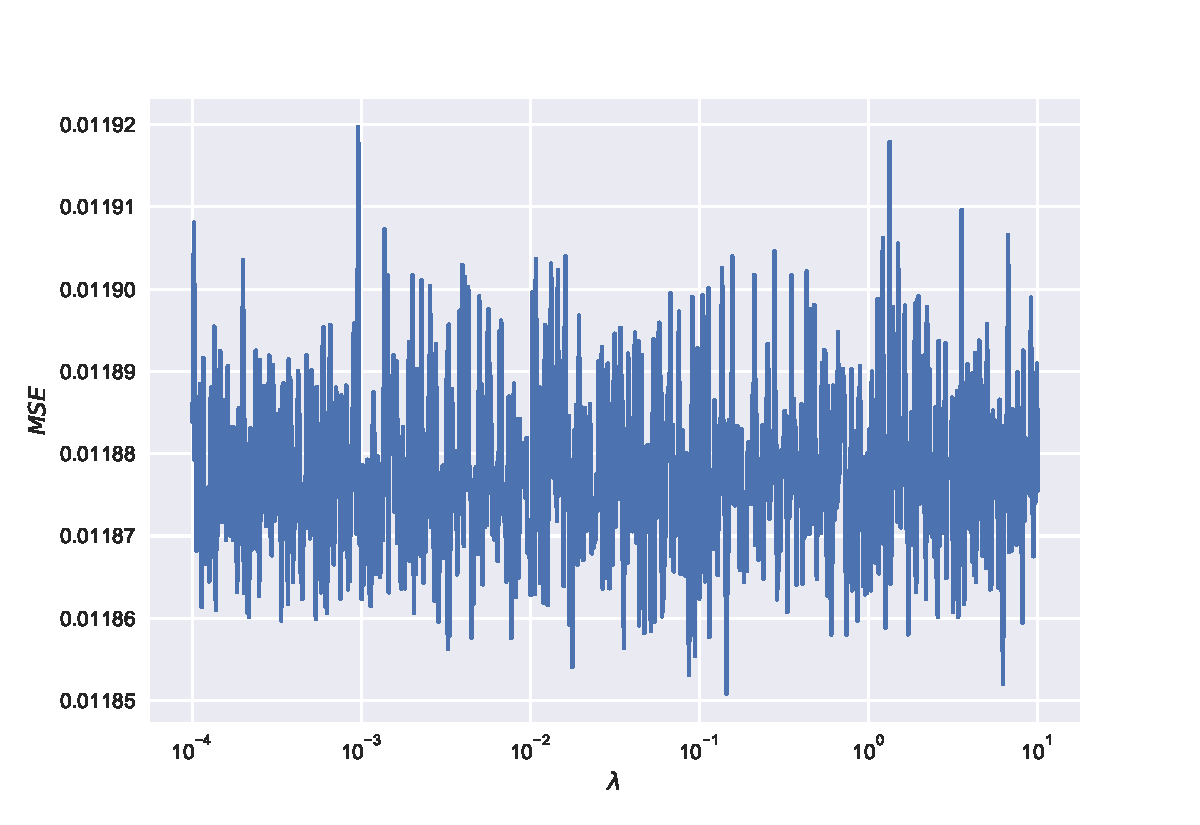
\includegraphics[scale=0.6]{../results/part_e_reg_MSE.pdf}
	\caption{The Mean Squared Error for the Lasso method for different values of $\lambda$}
	%Label gjør det enkelt å referere til ulike bilder.
	\label{part_e_MSE}
\end{figure}

\begin{figure}[h!]
	\centering 
	%Scale angir størrelsen på bildet. Bildefilen må ligge i %samme mappe som tex-filen. 
	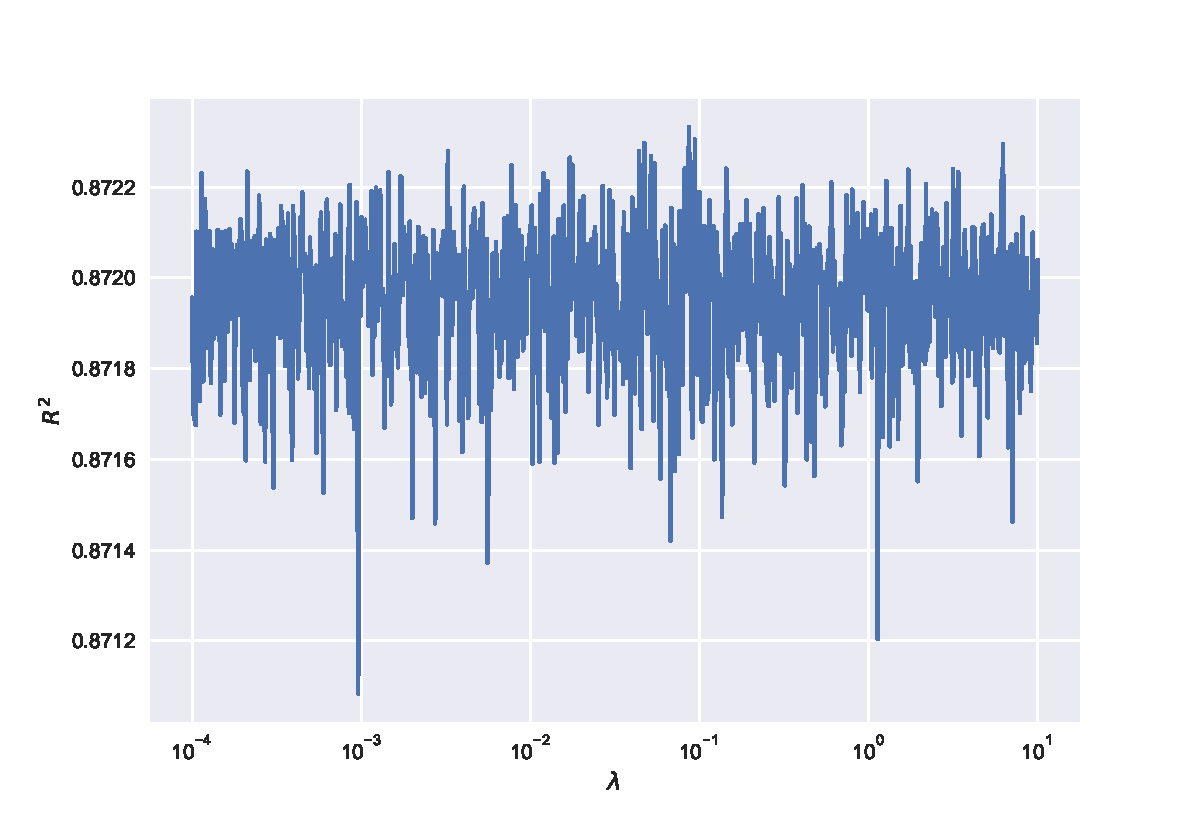
\includegraphics[scale=0.6]{../results/part_e_reg_R2.pdf}
	\caption{$R^2$-score for the Lasso method for different values of $\lambda$}
	%Label gjør det enkelt å referere til ulike bilder.
	\label{part_e_R2}
\end{figure}

%part g

\begin{figure}[h!]
	\centering 
	%Scale angir størrelsen på bildet. Bildefilen må ligge i %samme mappe som tex-filen. 
	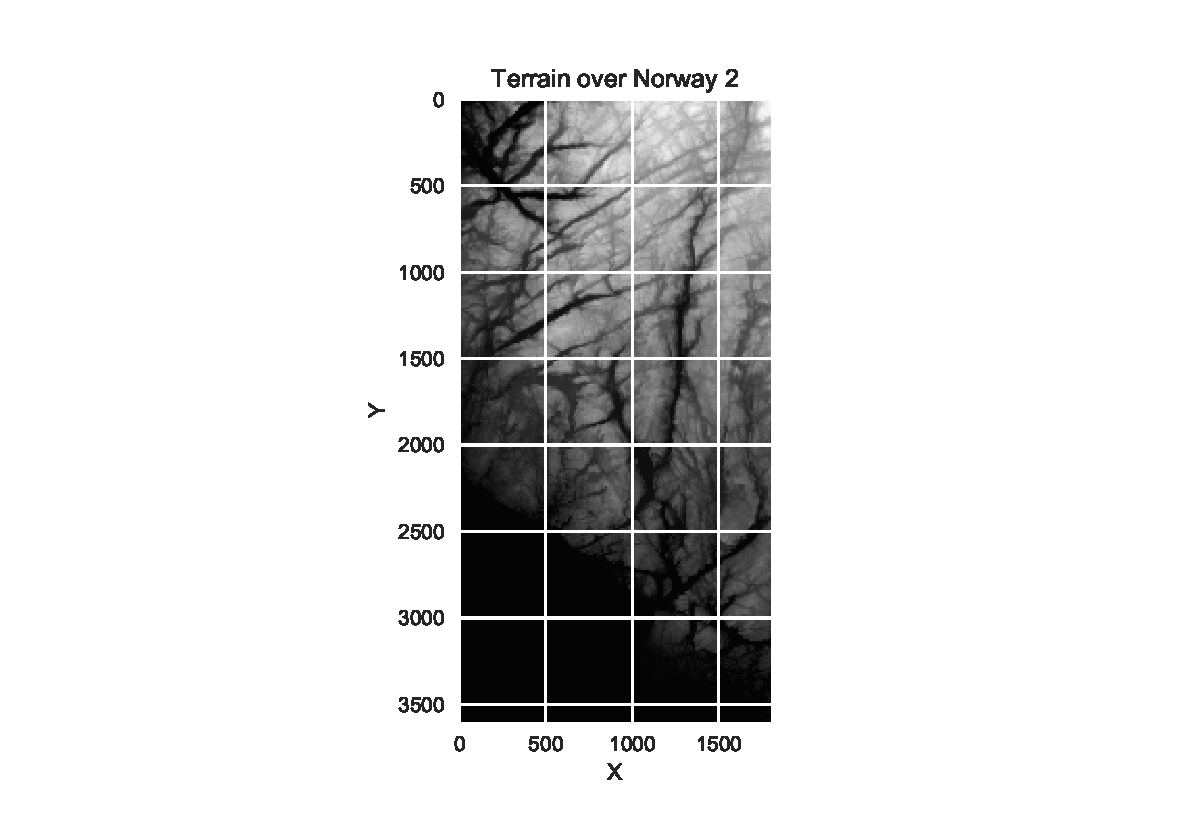
\includegraphics[scale=0.52]{../results/part_g_input.pdf}
	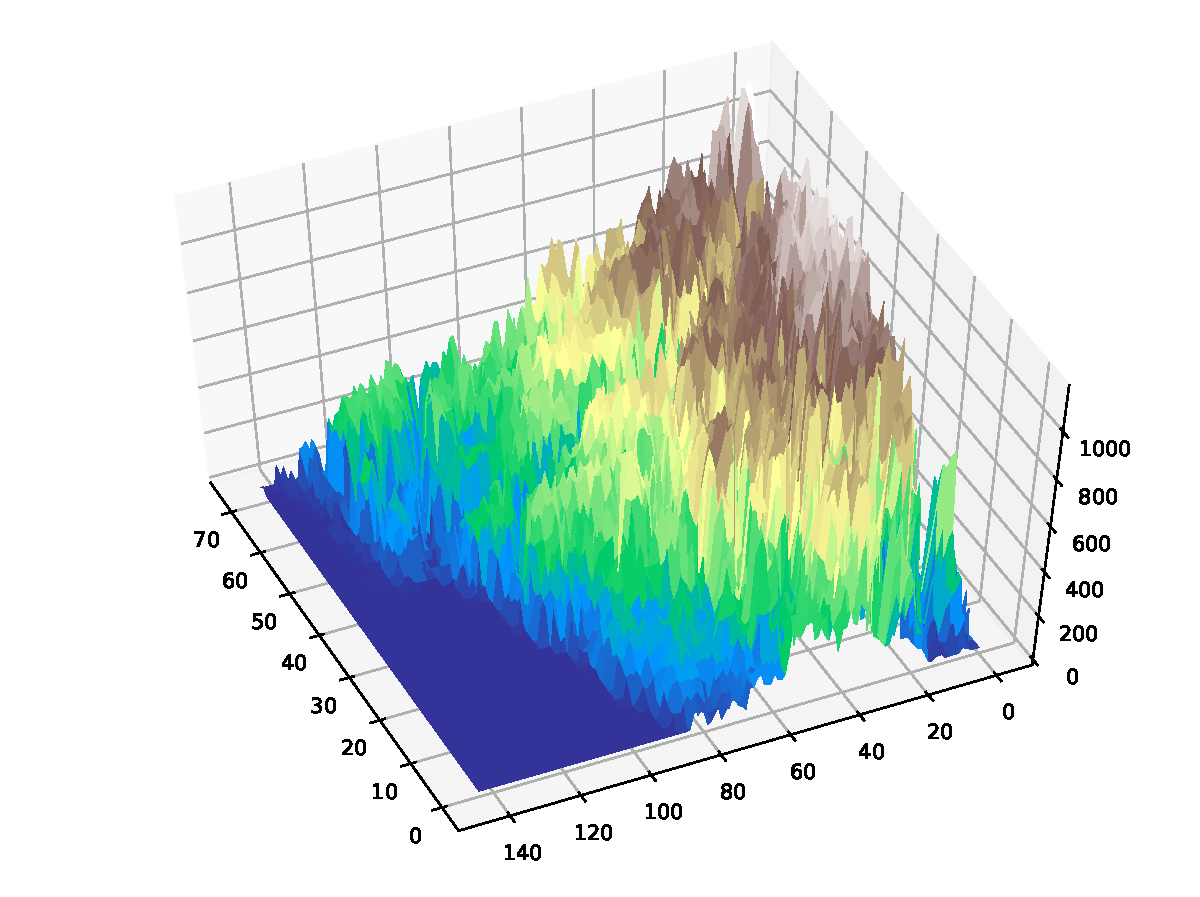
\includegraphics[scale=0.52]{../results/part_g_input3d.pdf}
	\caption{The terrain-data we are studying, from Møsvatn Austfjell in Norway}
	%Label gjør det enkelt å referere til ulike bilder.
	\label{part_g_input}
\end{figure}



%\begin{figure}[h!]
%	\centering 
%	%Scale angir størrelsen på bildet. Bildefilen må ligge i %samme mappe som tex-filen. 
%	\includegraphics[scale=0.6]{plot.pdf}
%	\caption{A plot of $PL$ against the dimensionless temperature $T_k$, using both the model for a large and small $T$	}
%	%Label gjør det enkelt å referere til ulike bilder.
%	\label{plot}
%\end{figure}


\section{Discussion}
\label{sec:discussion}

\newpage

\section{Appendix}
\label{sec:appendix}
	
\subsection{Part c math}

We are too show that 
\begin{align}
C(\boldsymbol{X}, \boldsymbol{\beta})=\frac{1}{n} \sum_{i=0}^{n-1}\left(y_{i}-\tilde{y}_{i}\right)^{2}
= \mathbf{E}\left[(\boldsymbol{y}-\tilde{\boldsymbol{y}})^{2}\right]
=\frac{1}{n} \sum_{i}\left(f_{i}-\mathbf{E}[\tilde{\boldsymbol{y}}]\right)^{2}+\frac{1}{n} \sum_{i}\left(\tilde{y}_{i}-\mathbf{E}[\tilde{\boldsymbol{y}}]\right)^{2}+\sigma^{2}
\end{align}

\begin{align}
\mathbf{E}\left[(\boldsymbol{y}-\tilde{\boldsymbol{y}})^{2}\right] 
=& \frac{1}{n} \sum_{i} \left( y_i - \tilde{y}_i \right)^2
= \frac{1}{n} \sum_{i} \left( f_i + \varepsilon - \tilde{y}_i \right)^2 \\
=& \frac{1}{n} \sum_{i} \left( f_i + \varepsilon - \tilde{y}_i  + \mathbf{E}[\tilde{\boldsymbol{y}}] - \mathbf{E}[\tilde{\boldsymbol{y}}] \right)^2 \hspace{0.9cm} 
| \hspace{0.1cm} \text{introduce $a = f_i - \mathbf{E}[\tilde{\boldsymbol{y}}] $ and $b = \tilde{y}_i - \mathbf{E}[\tilde{\boldsymbol{y}}]$}\\
=& \frac{1}{n} \sum_{i} \left( a - b + \varepsilon \right)^2
= \frac{1}{n} \sum_{i} \left( a^2 - 2ab + b^2 - 2b\varepsilon + \varepsilon^2 + 2a\varepsilon \right)\\
=& \frac{1}{n} \sum_{i} \left( f_i - \mathbf{E}[\tilde{\boldsymbol{y}}] \right)^2 
+ \frac{1}{n} \sum_{i} \left( \varepsilon^2 \right)
+ \frac{1}{n} \sum_{i} \left( \tilde{y}_i - \mathbf{E}[\tilde{\boldsymbol{y}}] \right)^2 
- 2\frac{1}{n} \sum_{i} \varepsilon \left( \tilde{y}_i - \mathbf{E}[\tilde{\boldsymbol{y}}] \right)
+ 2\frac{1}{n} \sum_{i} \varepsilon \left( f_i - \mathbf{E}[\tilde{\boldsymbol{y}}] \right)\\
&- 2\frac{1}{n} \sum_{i} \left( f_i - \mathbf{E}[\tilde{\boldsymbol{y}}] \right) \left( \tilde{y}_i - \mathbf{E}[\tilde{\boldsymbol{y}}] \right)\\
=& \frac{1}{n} \sum_{i} \left( f_i - \mathbf{E}[\tilde{\boldsymbol{y}}] \right)^2 
+ \frac{1}{n} \sum_{i} \left( \tilde{y}_i - \mathbf{E}[\tilde{\boldsymbol{y}}] \right)^2 
+ \sigma^2
- 2 \mathbf{E}[\varepsilon] \frac{1}{n} \sum_{i} \left( \tilde{y}_i - \mathbf{E}[\tilde{\boldsymbol{y}}] \right)
+ 2 \mathbf{E}[\varepsilon] \frac{1}{n} \sum_{i} \left( f_i - \mathbf{E}[\tilde{\boldsymbol{y}}] \right)\\
&- 2\frac{1}{n} \sum_{i} \left( f_i - \mathbf{E}[\tilde{\boldsymbol{y}}] \right) \left( \tilde{y}_i - \mathbf{E}[\tilde{\boldsymbol{y}}] \right)\\
=& \frac{1}{n} \sum_{i} \left( f_i - \mathbf{E}[\tilde{\boldsymbol{y}}] \right)^2 
+ \frac{1}{n} \sum_{i} \left( \tilde{y}_i - \mathbf{E}[\tilde{\boldsymbol{y}}] \right)^2 
+ \sigma^2 \hspace{0.3cm} \blacksquare
\end{align}

Where $\frac{1}{n} \sum_{i} \left( f_i - \mathbf{E}[\tilde{\boldsymbol{y}}] \right)$ is the bias and
$\frac{1}{n} \sum_{i} \left( \tilde{y}_i - \mathbf{E}[\tilde{\boldsymbol{y}}] \right)^2$ is the variance. 

(skal vi gjøre noe annet og?)



\end{document}




